\documentclass[12pt,letterpaper]{article}
\usepackage[margin=1in]{geometry}

\usepackage[utf8]{inputenc}
\usepackage[english]{babel}

\usepackage{siunitx}

\usepackage{natbib}
\usepackage[nottoc]{tocbibind}

\usepackage{xcolor}
\usepackage{listings}

\usepackage[T1]{fontenc}
\usepackage{mathptmx}

\usepackage{graphicx}
\usepackage{float}

\usepackage{appendix}

\usepackage{array}
\usepackage{tabulary}
\usepackage{multirow}

\usepackage{hyperref}
\hypersetup{
  colorlinks,
  citecolor=black,
  filecolor=black,
  linkcolor=black,
  urlcolor=black
}

\begin{document}
\begin{center}
  {\scshape\Large HamSCI: Eclipse Simulator Documentation\par}
  \vspace{1em}
  {\large Joshua S. Vega, WB2JSV\par}
  \vspace{1em}
  {\itshape\large Last Updated: \today\par}
\end{center}

\tableofcontents

\newpage

%
% INTRODUCTION
%
\section{Introduction}
\label{sec:introduction}

HamSCI's eclipse simulator (colloquially known as ``\texttt{eclipsesim}'') is a
software package developed by members of the HamSCI team at the New Jersey
Institute of Technology used to simulate HF (3-30 $\si{\mega\hertz}$) through
the ionosphere. Specifically, the package was developed in order to simulate the
effects of the August 21, 2017 total solar eclipse on HF amateur ``ham'' radio
communications. The bulk of the package is developed in MATLAB. However, the
inputs and outputs are both in the comma-separated values (CSV) format in order
to allow for easy interoperability with other analysis tools (such as those
written in Python, R, or Julia).

This document is written in order to provide the reader with an understand of
the inner workings of the simulation package as well as justify some of the
design decisions that were made during development. In addition, this document
is intended to be used as a helpful guide to using the package. Because of this,
as the package undergoes future changes, so too should this document in order to
maintain parity between the package and its documentation.

%
% DEPENDENCIES
%
\section{Dependencies}
\label{sec:dependencies}

The \texttt{eclipsesim} package relies on a few third-party dependencies in
order to implement some specialized functionality. This section provides a brief
overview of the different dependencies and their function.

\subsection{PHaRLAP}
\label{sec:dependencies:pharlap}

PHaRLAP\footnotemark is a robust HF raytracing toolkit developed by Dr. Manuel
Cervera of the Defence Science and Technology Group, Australia. It is used to
compute the actual ray paths of radio transmission from transmitter to
receiver. More information on how it is used is provided in
\autoref{sec:design}. Although the core of the toolkit is written in FORTRAN, a
MATLAB application programming interface (API) is provided. PHaRLAP also
provides a simple API for the IRI (see below) that is compatible with the ray
path computation API.

\footnotetext{\itshape``The results published in this paper were obtained using
  the HF propagation toolbox, PHaRLAP, created by Dr. Manuel Cervera, Defence
  Science and Technology Group, Australia
  (manuel.cervera@dsto.defence.gov.au). This toolbox is available by request
  from its author.''}

% \subsection{IRI}
% \label{sec:dependencies:iri}

% The International Reference Ionosphere (IRI)\footnotemark is a ionospheric model
% developed by the Committee on Space Research (COSPAR) and International Union of
% Radio Science (URSI). It is periodically updated to incorporate new
% measurements. It generates monthly averages for several ionospheric measurements
% including electron density, and electron and ion temperatures.

% \footnotetext{\url{http://irimodel.org/}}

\subsection{SAMI3}
\label{sec:dependencies:sami3}

SAMI3 is a three-dimensional global ionosphere model developed by the U.S. Naval
Research Laboratory (NRL). In 2017, Joseph D. Huba and Douglas Drob published a
paper detailing a modified SAMI3 model that simulated effects of the August 21,
2017 eclipse on the ionosphere \citep{Huba2017}. This model was provided to
HamSCI by Joseph Huba and have since been the {\it de facto} ionosphere model
for eclipse simulations. For more information on SAMI3's data structure and how
it has been integrated into the eclipse simulation, see
\hyperref[sec:sami3_df]{Appendix B}.

%
% USAGE
%
\section{Usage}
\label{sec:usage}

The \texttt{eclipsesim} package provides two methods of execution
out-of-the-box: serially and in parallel. More information and specific
instructions on each execution method is discussed in \autoref{sec:usage:serial}
and \autoref{sec:usage:parallel}, respectively.

Regardless of the execution method used, \texttt{eclipsesim} is designed to be
executed on a Linux-based machine. While limited success has been achieved on
other operating systems (notably, Microsoft Windows), the execution scripts are
developed with Linux in mind and may not execute as expected in incompatible
environments. All instructions provided in this section are therefore intended
for Linux-based systems and may require modification for other operating
systems.

\subsection{Setup}
\label{sec:usage:setup}

Before the eclipse simulation can be run, all external dependencies must be
accessible to the simulation program. This section briefly describes what
dependencies are required and how they must be configured. Some extension
version of the simulation program may require additional dependencies. Please
refer to \hyperref[sec:extensions]{Appendix A} for extension-specific dependency
information.

{\bf MATLAB}: Since all computation is executed in MATLAB, it should come as no
surprise that the most important dependency is MATLAB itself. The simulation is
primarily designed to execute on version 2016a however later versions should
also be compatible. When using older versions of MATLAB some compilation and
runtime errors have been seen to occur due to breaking changes between older
version and 2016a or later. Once MATLAB has been installed, it's important to
ensure that the {\tt matlab} program is available for execution through a
modified {\tt \$PATH} variable.

{\bf PHaRLAP}: As described in \autoref{sec:dependencies:pharlap}, PHaRLAP is a
vital part of the simulation program. Due to the restrictions on the
distribution of PHaRLAP, it is not and should not be directly distributed with
any of the eclipse simulation versions. Instead, it is recommended that
prospective users of the simulation tool contant the author of PHaRLAP and
receive a direct copy. Once a copy of PHaRLAP is acquired, it can be installed
anywhere that is accessible to the simulation tool as long as the {\tt
  PHARLAP\_DIR} variable is updated appropriately in the execution script.

% {\bf IRI}: If the IRI will be used as the ionosphere model there is no need to
% install any additional dependencies as it is already integrated into
% PHaRLAP. However, keep in mind that with most version of the simulation tool
% being designed for SAMI3, some modification of the simulation code will be
% required.

{\bf SAMI3}: If SAMI3 will be used as the ionosphere model, then there are a few
steps required in order to prepare it to work with the simulation tool. After
acquiring the SAMI3 model it must be converted from the raw data format to the
{\tt *.m} file format which is far more efficient for MATLAB to load and
parse. For detailed information about this step, refer to
\hyperref[sec:sami3_df]{Appendix B}. Once it has been properly converted, the
SAMI3 {\tt *.m} file(s) must be placed in a directory that is accessible to the
simulation program. Be sure to update the {\tt SAMI3\_PATH} variable
appropriately in the execution script.

\subsection{Serial}
\label{sec:usage:serial}

The serial execution model is designed for testing or very short
simulations. The serial execution model only executes the simulation for a
single point in time. This can obviously be adjusted by modifying the bash
execution script. However for this sample, it is assumed that only one time-step
is being simulated. It is also assumed that all dependencies have been properly
installed and configured and that the appropriate modifications have been made
to the execution script.

To execute the simulation tool in serial mode, you'll be executing the {\tt
  eclipsesim\_local.sh} file in as bash script without any arguments (ensure
that it has been configured to have the execution permissions bit enabled):

\begin{lstlisting}[language=bash]
  $ ./eclipsesim_local.sh
\end{lstlisting}

This script will the first job file available in the input directory (see
\autoref{sec:usage:input} for information on inputting data to the simulation
tool). When the simulation is complete the terminal will be prepared for a new
command and the outputted data will be available in the output directory (see
\autoref{sec:usage:output} for information on outputting data from the
simulation tool). If an error occured during the simulation, MATLAB will halt
and indicate where in the MATLAB code the error occurred.

\subsection{Parallel}
\label{sec:usage:parallel}

The parallel execution model is designed to be executed on a computing cluster
running a Sun Grid Engine (SGE; now Oracle Grid Engine) compatible scheduling
system. One such system is Son of Grid Engine (also SGE). When submitting a job,
SGE adds it to the job queue. When a compute node with the requested resources
is made available, the next job is assigned to be executed on said node. SGE
also allows multiple compute nodes to be requested by one job using the array
option. For more information about the many options made available to jobs,
please refer to both the SGE documentation as well as any cluster-specific
documentation.

To execute the simulation tool in parallel mode, execute the {\tt
  eclipsesim\_sge.sh} file as an argument to the {\tt qsub} application.

\begin{lstlisting}[language=bash]
  $ qsub ./eclipsesim_sge.sh
\end{lstlisting}

This command will submit the job file to the SGE queue. Once the job has been
selected for execution, it will ensure that MATLAB is loaded and then begin the
process of preparing the simulation for execution (this step is identical to the
equivalent step in the serial execution model). Due to the parallel nature of
this execution model, no response will be printed to the terminal. Instead, a
log file for each job submitted job (if the job is an array job, one log file
will be generated for each sub-job) containing all output information for that
individual job (or sub-job). For this reason it is not recommended that the
simulation be tested or debugged in the parallel execution mode (unless it is
directly related to the parallel nature of the execution).

\subsection{Input}
\label{sec:usage:input}

In order for the simulation tool to execute, it requires some input data. This
data is usually in the form of a transmitting station location, receiving
station location, frequency, and time of exchange. Because the simultion is
divided into timestamps, the time of exchange is encoded into the input
filename. This is done using the format {\tt ``<YYYY>-<MM>-<DD>
  <HH>:<mm>:<ss>.csv''} (e.g. {\tt ``2017-08-21 16:00:00.csv''} for August 21,
2017 at 4:00 PM UTC).

Within the input file, the remainder of the input data is stored. This is done
by entering the data as rows into the file using the Comma-Separated Values
(CSV) format. The first line of file should be {\tt
  ``RX\_CALL,TX\_CALL,MHZ,RX\_LAT,RX\_LON,TX\_LAT,TX\_LON''}. \autoref{tbl:input_fields}
shows the different input fields (all fields are required).

\begin{table}
  \centering
  
  \begin{tabulary}{\linewidth}{| L | L | L | L |}
    \hline
    {\bf Name} & {\bf Datatype} & {\bf Description} & {\bf Example}\\\hline
    {\tt RX\_CALL} & \multirow{2}{*}{alphanumeric string} & The name (or callsign) of the RX station. & {\tt WE9V}\\\cline{1-1}\cline{3-4}
    {\tt TX\_CALL} &                                      & The name (or callsign) of the TX station. & {\tt N8PW}\\\hline
    {\tt MHZ} & \multirow{5}{*}{floating-point number} & The frequency of the transmission in $\si{\mega\hertz}$. & {\tt 7.03}\\\cline{1-1}\cline{3-4}
    {\tt RX\_LAT} &                                    & The latitude of the RX station. & {\tt 42.5625}\\\cline{1-1}\cline{3-4}
    {\tt RX\_LON} &                                    & The longitude of the RX station. & {\tt -88.0417}\\\cline{1-1}\cline{3-4}
    {\tt TX\_LAT} &                                    & The latitude of the TX station. & {\tt 40.8542}\\\cline{1-1}\cline{3-4}
    {\tt TX\_LON} &                                    & The longitude of the TX station. & {\tt -81.3750}\\\hline
  \end{tabulary}

  \caption{The input data fields for the simulation.}
  \label{tbl:input_fields}
\end{table}

Below is an example row from an input file:

\begin{center}
  {\tt WE9V,N8PW,7.03,42.5625,-88.0417,40.8542,-81.3750}
\end{center}

Once the correct input files have been created (or possibly generated), they
should be placed into the {\tt ./jobs} sub-directory of the simulation tool's
directory.

\subsection{Output}
\label{sec:usage:output}

PHaRLAP outputs a wide array of simulation values for each simulated
ray. However, for the purposes of this simulation tool, only the values related
to the ``best'' ray-path between the transmitting station and receiving station
are taken into account. Yet still there are many outputted values that are
recorded into the output CSV files. \autoref{tbl:output_fields} details them.

\begin{table}
  \centering

  \begin{tabulary}{\textwidth}{| L | p{20em} |}
    \hline
    
    %
    % Station Information
    %
    {\tt tx\_call} & The name (or callsign) of the TX station.\\\hline
    {\tt rx\_call} & The name (or callsign) o fthe RX station.\\\hline
    {\tt tx\_lat} & The latitude of the TX station.\\\hline
    {\tt tx\_lon} & The longitude of the TX station.\\\hline
    {\tt rx\_lat} & The latitude of the RX station.\\\hline
    {\tt rx\_lon} & The longitude of the RX station.\\\hline
    {\tt freq} & The frequency of the transmission in $\si{\mega\hertz}$.\\\hline

    %
    % Simulation Results
    %
    {\tt srch\_rd\_lat} & The latitude of the end point of the ray.\\\hline
    {\tt srch\_rd\_lon} & The longitude of the end point of the ray.\\\hline
    {\tt srch\_rd\_ground\_range} & The ground range of the ray in $\si{\kilo\meter}$.\\\hline
    {\tt srch\_rd\_group\_range} & The group range of the ray in $\si{\kilo\meter}$.\\\hline
    {\tt srch\_rd\_phase\_path} & The phase path of the ray in $\si{\kilo\meter}$\\\hline
    {\tt srch\_rd\_geometric\_path\_length} & The physical distance along ray path in $\si{\kilo\meter}$.\\\hline
    {\tt srch\_rd\_initial\_elev} & The initial elevation of this hop in degrees.\\\hline
    {\tt srch\_rd\_final\_elev} & The final elevation of this hop in degrees.\\\hline
    {\tt srch\_rd\_apogee} & The maximum altitude of the ray in $\si{\kilo\meter}$.\\\hline
    {\tt srch\_rd\_gnd\_rng\_to\_apogee} & The ground range to the apogee in $\si{\kilo\meter}$.\\\hline
    {\tt srch\_rd\_plasma\_freq\_at\_apogee} & The plasma frequency at the ray apogee $\si{\mega\hertz}$.\\\hline
    {\tt srch\_rd\_virtual\_height} & The virtual height of the ray in $\si{\kilo\meter}$.\\\hline
    {\tt srch\_rd\_effective\_range} & The effective range of the ray in $\si{\meter}$.\\\hline
    {\tt srch\_rd\_deviative\_absorption} & The ionospheric deviative absorption in dB.\\\hline
    \multirow{2}{*}{\tt srch\_rd\_TEC\_path} & The integrated electron density along the ray path (number of electrons in $\SI{1}{\square\meter}$ cross-section tube).\\\hline
    {\tt srch\_rd\_Doppler\_shift} & The Doppler shift in $\si{\hertz}$.\\\hline
    {\tt srch\_rd\_Doppler\_spread} & The Doppler spread in $\si{\hertz}$.\\\hline
    \multirow{2}{*}{\tt srch\_rd\_FAI\_backscatter\_loss} & The backscatter loss in dB for the last hop due to field aligned irregularities.\\\hline
    {\tt srch\_rd\_frequency} & The carrier frequency used for the ray.\\\hline
    {\tt srch\_rd\_nhops\_attempted} & The number of hops in this ray.\\\hline
    {\tt srch\_rd\_rx\_power\_0\_dB} & \multirow{4}{*}{\it These fields should be ignored.}\\\cline{1-1}
    {\tt srch\_rd\_rx\_power\_dB} & \\\cline{1-1}
    {\tt srch\_rd\_rx\_power\_O\_dB} & \\\cline{1-1}
    {\tt srch\_rd\_rx\_power\_X\_dB} & \\\hline
    {\tt srch\_rd\_hop\_idx} & The index for this hop.\\\hline
    {\tt srch\_rd\_apogee\_lat} & The latitude of the apogee.\\\hline
    {\tt srch\_rd\_apogee\_lon} & The longitude of the apogee.\\\hline
  \end{tabulary}

  \caption{The output data fields for the simulation.}
  \label{tbl:output_fields}
\end{table}

These output files will be located in the directory specified by the {\tt
  OUT\_PATH} variable in the execution directory (ensure that this directory
exists prior to execution or else the simulation will crash). The filename
indicates the time at which the simulation was executed using the form {\tt
  ``simulated\_<YYYY>-<MM>-<DD>\_<HH>-<mm>.csv''} (e.g. {\tt
  ``simulated\_2017-08-21\_16-00.csv''} for August 21, 2017 at 4:00 PM UTC).

It's important to remember that each row is not a unique ray-trace. Instead, a
row only provides the information relevant to a single hop of a
ray-trace. Therefore, if for example a ray required 3 hops to travel the
distance between the transmitter and receiver then 3 rows will appear in the
output file. In this case, the {\tt srch\_rd\_hop\_idx} field will indicate the
order in which the hops occurred (e.g. 1 being the first hop and 3 being the
last). In this case, it's also important to realize that the field {\tt
  srch\_rd\_nhops\_attempted} is not necessarily the number of resulting number
of rows that will appear in the output file. If the maximum number of hops is
set at 10 for example but if only 3 hops are needed then only 3 rows will appear
for that ray-trace.

%
% DESIGN
%
\section{Design}
\label{sec:design}

This section discusses the inner-workings of the eclipse simulator
package. However, it does not discuss how PHaRLAP or any other dependency
function and instead focuses on how such functionality is being used. Please
refer to the respective documentation for design details about any dependencies.

\subsection{Rough Pass}
\label{sec:design:rough}

The most basic functionality of the eclipse simulator package is the initial
raytrace calculation. Here, PHaRLAP is used to raytrace several ray paths at
different takeoff angles (the initial angle above the horizon from the
transmitting station). For a usual simulation, the rays are lauched at
$\SI{0.5}{\degree}$ increments from $\SI{5}{\degree}$ to
$\SI{60}{\degree}$. Each ray is simulated for 3 hops. From this set of rays, it
is possible to determine at which takeoff angle and hop count the ray landed
closest to the receiver. Two rays are selected: the closest ray that landed
before the receiver, and the closest ray that landed beyond the receiver. These
two rays are the boundaries for the ``Fine Pass'' described in
\autoref{sec:design:fine}.

\subsection{Fine Pass}
\label{sec:design:fine}

The fine pass works very similarly to the rough pass. Asside from the boundaries
set by the rough pass, the fine pass is also distinct in that it iterates using
an increment that is a fifth of the difference between that of the two
bracketing rays (e.g. if the selected rays have takeoff angles of
$\SI{10}{\degree}$ and $\SI{10.5}{\degree}$, then the new inrecment would be
$\SI{0.1}{\degree}$. It is assumed that the two selected takeoff angles are
within twice the rough increment step from one another (when the rough increment
is $\SI{0.5}{\degree}$, the difference in takeoff angles cannot be more than
$\SI{1}{\degree}$).

After the fine pass has been raytraced, linear interpolation is used to finally
find the ``best'' take-off angle for a transmission between a transmitter and
receiver. The raytracer is executed with this ``best'' takeoff angle and the
outputted values are saved to the output CSV file in the format described in
\autoref{sec:usage:output}.

\subsection{Plotting}
\label{sec:design:plotting}

Plotting is the final major step in the simulation
program. \autoref{fig:raytrace-sample} shows a sample ray trace plot generated
by the simulation tool. The y-axis represents the altitude from sea level and
the x-axis represents the ground range beginning at the transmitter in the
direction of the reciever. In this plot, we see the raytrace of the ``best''
takeoff angle highlighted in red while the remaining ray-traces are shown in
white. The background of the plot represents the Plasma frequency as taken from
SAMI3 in order to demonstrate where the different ionospheric layers reside. The
plot is also curved in order to ensure that the ray is properly shown as being
traced over the horizon. Note that this specific raytrace was done for a single
hop scenario in which the ground range is relatively short.

Although not demonstrated in this plot, it is important to recall that the
ground is represented as a prefectly smooth reflector. Therefore, the angle of
reflection will always be equal to the angle incidence. Diffusion and
attenuation based on ground composition is not natively supported in PHaRLAP and
has not been implemented into the simulation itself as of writing.

\begin{figure}
  \centering

  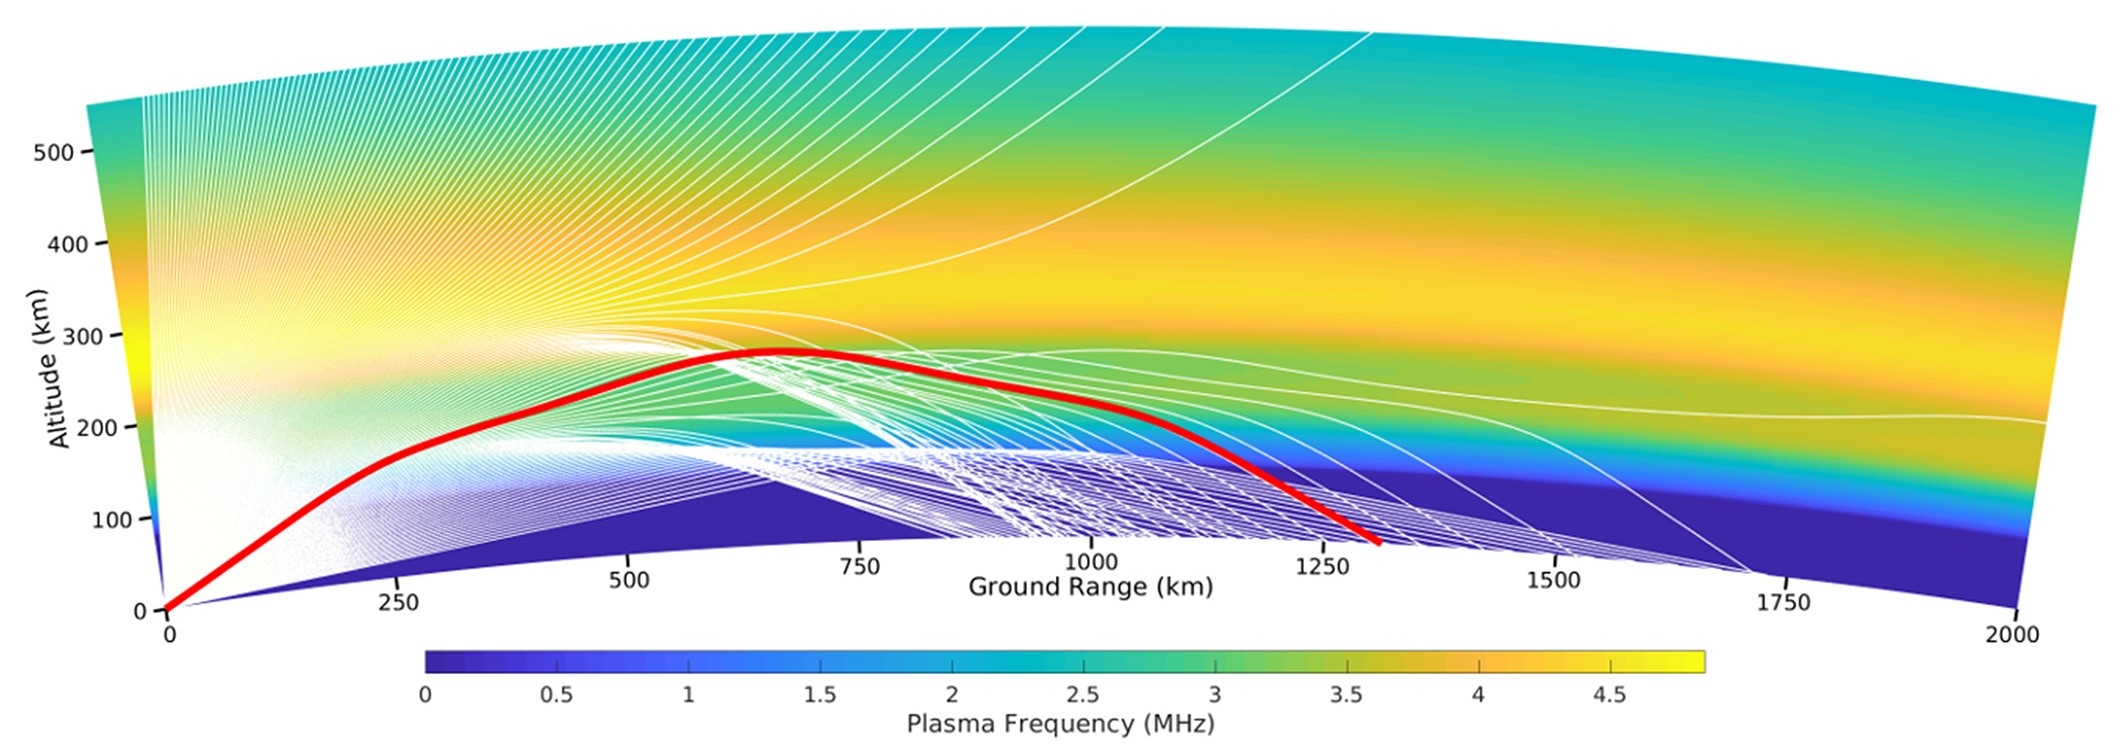
\includegraphics[width=\linewidth]{raytrace-sample}

  \caption{A sample raytrace plot.}
  \label{fig:raytrace-sample}
\end{figure}

%
% CONCLUSION
%
\section{Conclusion}
\label{sec:conclusion}

This document is an attempt to describe the inner-workings and reasoning behind
the decision made when developing the eclipse simulation tool. While it attempts
to be as comprehensive as necessary it assumes that the reader is comfortable
reading code and has a basic understanding of ionospheric science.

Although the simulation was initially developed for the August 21, 2017 solar
eclipse and focused on the simulation of amateur ``ham'' radio communications,
the concepts behind it are fairly generic and thus can similarly be applied to
any number of ionospheric simulations.

The simulation itself is still being actively developed thus there are features
not discussed in this document that may be added in later versions of the
simulation program. The program itself does not maintain any sort of regular
release cycle and new features are added in an ``as-needed'' basis. Because of
this, this document is not intended as a definitive and comprehensive
description of the simulation program. Rather, it is merely intended as an
introduction and should be accompanied with actively reading of the MATLAB code
and experimentation with the program.

%
% REFERENCES
%
\pagebreak
\renewcommand{\bibname}{References}
\bibliographystyle{abbrvnat}
\bibliography{eclipsesim}

\newpage
\begin{appendices}
  
  % 
  % SAMI3 DATA FORMAT
  % 
  \section{Appendix: SAMI3 Data Format}
  \label{sec:sami3_df}

  {\it To be written \dots}

\end{appendices}

\end{document}